\ofsubsection{Bestiary}
%
\ofquote{"With each passing day, the world finds new and exciting ways to kill a man."}{Balthier}
%
\\\\
%

\includegraphics[width=\columnwidth]{./art/images/ff6.jpg}
%
\vfill
%
\accf{Combat Encounters} can occur in many different situations, for example, the party might try to drive away a gang of bandits or they might face their main antagonist in an epic showdown.
Combat is usually a matter of life and death and it can take up a significant portion of your playtime.
However, it does not always have to be a fight till death, but the party may seek out alternative resolutions such as negotiation or escape.
During combat, you as the GM take the role of all adversaries and the regular combat rules apply to them, but you may keep some crucial information secret, such as attributes and dice rolls of enemies.
While playing as an enemy party, try to make decisions from their perspective without using your own knowledge.
In addition, it is also helpful to use visual aids like maps to keep track of the battlefield.
\accf{Combat Rewards} often make up a major portion of the party's wealth and the table below provides a rough guideline depending on the party Level.
A party with insufficient Gil cannot afford essential items, but one with too much money can avoid too many consequences.
Rewards do not always have be in Gil, but can also be equipment, items or materials of similar value and by default they are divided between all party members.
%
\vfill
%
\oftable{p{0.3\columnwidth} p{0.7\columnwidth}}
{\accf{Level} & \accf{Combat Reward per Player}}
{
	1 & 200G \ofrow
	2 & 300G \ofrow
	3 & 500G \ofrow
	4 & 800G \ofrow
	5 & 1000G \ofrow
	6 & 1200G \ofrow
	7 & 1500G \ofrow
	8 & 2000G \ofrow
	9 & 2500G \ofrow
	10 & 3000G
}
%
\newpage
%
The difficulty of combat encounters can vary greatly and you can tune it depending on the context and your group's preferences.
On the one hand, combat is the most common cause of character death, so we recommend some caution to avoid unexpected surprises.  
On the other hand, you usually want combat to be a respectable challenge for the party.
Finding a pleasant balance might take some effort, because the difficulty of an encounter depends on a many factors:
first, the circumstances of a battle can heavily tip the scale.
For example, the players will be at a strong disadvantage when they have already suffered through other battles on the same day or when the other side gains a surprise round.
Furthermore, the composition and preparation of both parties has a great effect on the outcome.
For example, a party consisting only of melee fighters will have no issues with ordinary enemies, but will likely struggle against ones with ranged damage and Status Effects.
Finally, the experience of your group will also have a great impact.
For example, players who are new to the game are likely to miss opportunities, while ones with a lot of experience often have unexpected tricks up their sleeves.
All in all, we unfortunately cannot name any strict rules that apply to all groups and situations.
Nevertheless, we will discuss some rough guidelines and rules-of-thumb that you can take into consideration.
Note that we generally err on the side of caution with advice and prepared content and you are encouraged to modify them in case they do not provide you with sufficient challenge. 
%
\ofpar
%
When structuring an enemy party, we generally recommend to have similar participant counts on each side where each enemy is roughly equal in strength to a player character.
Large hordes of weaker enemies will often overwhelm the party, while lone ones rarely stand a chance.
A balanced setup ensures that two important resources are roughly equal: the number and strength of combat actions on both sides.
To gauge the strength of an enemy, we use Levels that we can compare against that of player characters.
For example if the player party consists of four Level 4 characters, the opposing party should contain an equal amount of enemies with the same Level.
As a next step, you can use the following guideline to determine their attributes: 
for every Level, an enemy gains 6 \accf{Attribute Points}, where each point is equal to maximum HP/MP~+5 or STR/MAG/DEF/RES~+1.
Their AGI should usually range between 1 and 4, otherwise regular Attacks will become very ineffective.
Just like characters, enemies can use Magic and Techs, as well Passive and Reaction abilities.
However, we recommend to keep the number of enemy abilities low to allow for quick decisions during combat.
Still, you can feel free to give them access to unique and exotic abilities.
We consider any equipment in the total attributes of an enemy and for weapons we assign the DMG of the equipment rank appropriate to the enemy's Level.
You can also add more depth to enemies by assigning elemental resiliences and weaknesses or status effect immunities.
During combat, you can give subtle hints about these specialties to the players when narrating combat actions and their effects.
%
\vfill
%
In some cases, it can be more interesting to create an opposing party that is unbalanced in participant count.
For example, you might want the party to face a horde of weaker enemies or a singular strong enemy, a so-called \accf{Boss}.
Accordingly, in those cases, the strength of enemies will differ from those of the player characters.
In case the enemy party outnumbers the players, we recommend to use lower Level enemies such that the sum of all Levels is roughly equal for both parties.
In case an enemy is outnumbered, he needs additional strength to handle multiple adversaries.
Apart from increased attributes, \accf{Boss Traits} can help your Bosses to make up for their lack of numbers.
Boss Traits are particularly strong special abilities that grant enemies additional actions and durability. 
We recommend the following guideline to balance n boss: for every additional adversary that a boss should be able to handle give them 2 extra Attribute Points per Level as well as one Boss Trait.
For example, a single Level 5 boss fighting against a party of 4 should have at least \mbox{5 x (6 + 3 x 2) = 60 Attribute Points} and 3 Boss Traits.
A list of Boss Traits is shown on the right hand side.
%
\vfill
%
The following types of irregularly balanced enemy party setups are commonly used:
\ofrow
\accf{Single Boss:}
A lone powerful enemy, this could for example be the main antagonist.
Use the above mentioned guideline to ensure that the boss can handle multiple player characters.
A single Boss also greatly benefits from additional specialties, such as special interactions with the environment.
This variant is the hardest balance, so we recommend to prefer other ones when possible.
\ofrow
\accf{Council Boss:} 
The enemy party consists of a small group of Bosses, usually 2 or 3.
Each of them is equally strong, but stronger than a player character.
Usually, their strengths complement each other, for example, one Boss might be focused on offense while the other excels at healing.
\ofrow
\accf{Boss with Minions:} 
This boss has several regular enemies working with them, for example a Necromancer raising her undead hordes. 
In this case, the Boss is stronger than a player character while the minions are weaker.
\ofrow
\accf{Multi-Part Boss:} 
This type of boss is represented by multiple parts.
Each part is built as one enemy with its own turn, attributes and abilities, but all parts can only move together at once.
Usually, one of the parts acts as the core, when it dies, all other parts die with it.
The core usually also has additional protection and the ability to regenerate other parts, once they suffer KO.
\ofrow
\accf{Enemy Horde:} 
A large group of regular enemies, usually each with the same type and a lower Level than a player character.  
However, we advise against outnumbering the party more than 2 to 1, for example if you have 4 players, they should not face more than 8 enemies at once.
%
\newpage
%
\oftable{p{0.24\columnwidth} p{0.7\columnwidth}}
{\accf{Boss Trait} & \accf{Effect}}
{
	Auto-Hit & You Attacks cannot be evaded but they also cannot be Critical Hits. \ofrow
	Auto-Blink & You permanently have Blink. \ofrow
	Auto-Haste & You permanently have Haste. \ofrow
	Auto-Regen & You permanently have Regen. \ofrow
	Auto-Quicken & You can take 2 turns per round. \ofrow
	All-Immune & You have permanent Immunity against all negative Status Effects. \ofrow
	Counter & Once per round, when you suffer damage, you can make an Attack against the perpetrator if he is in range. \ofrow
	CT-0 & All of your cast times of your spells and techs are reduced to 0r.\ofrow
	Dual Attack & With each Attack, you can target 2 different enemies in range. \ofrow
	Fade & You can evade Magic effects in the same way you evade Attacks. \ofrow
	Final Attack & When you suffer KO, you may take one action before falling unconscious. \ofrow
	Revert & Once per round, you may redo one of your die rolls after seeing its result. \ofrow 
	Retaliate & Once per round, when you suffer damage, you can use any ability against the him if he is in its range. \ofrow
	Surge & When current HP falls below half of its max., you gain EnSTR, EnDEF, EnMAG and EnRES until the end of battle. \ofrow
}
%
\vfill
%
\accf{Gladio: "So, this Blademaster..." \\ Cor: "He's a master of blades. What, were you expecting something profound?"}
%
\vfill
%
Apart from non-player characters, \accf{Monsters} are another common type of adversary that the party may face in combat. 
Monsters are wild beings that live in their natural habitats, upon contact with the party they usually feel threatened and attack.
Different monsters often work together against hostiles and the party might come across more intelligent monsters with complex goals.
They are often part or cause of major conflicts and thus your adventure may feature various monsters at the center of its plot. 
Compared to characters, monsters can also vary greatly in size and appearance.
They are classified as Medium~(\accf{M}) if they take up roughly 1u in diameter, as Large~(\accf{L}) if they take up more than 2u and as Small~(\accf{S}) if they take up less than 0.5u when viewed from above.
Monsters do not use regular weapons and armor, but they have equivalent parts integrated into their bodies, that follow the same rules.
The following pages include various prepared monsters of different Levels.
You may use them as given, but we also encourage you to modify them to suite your needs or use them as examples for creating your own.
%
\clearpage
%
%
%
%%%%%%%%%%%%%%%%%%%%%%%%%%%%%%%L1%%%%%%%%%%%%%%%%%%%%%%%%%%%%%%%%%%%%%%%%%
%
\ofmonster{Goblin}{1}{
\includegraphics[width=0.2\columnwidth]{./art/monsters/goblin.png}}
{
	HP: & \hfill 12 & MP: & \hfill 0\\
	STR: & \hfill 2 & DEF: & \hfill 1 \\
	MAG: & \hfill 0 & RES: & \hfill 1 \\
	AGI: & \hfill 3 & Size: & \hfill M\\
}
{\accf{Knife}: 1d DMG \hfill \accf{Immune}:\immobile}
{}
%
\vfill
%
\ofmonster{Skeleton}{1}{
\includegraphics[width=0.17\columnwidth]{./art/monsters/skeleton.png}}
{
	HP: & \hfill 11 & MP: & \hfill 0\\
	STR: & \hfill 2 & DEF: & \hfill 2 \\
	MAG: & \hfill 0 & RES: & \hfill 0 \\
	AGI: & \hfill 2 & Size: & \hfill M \\   
}
{\accf{Sword}: 1d DMG \hfill \accf{Weak}:\fire\holy}
{\mpassive{Undead}{You permamently suffer Zombie.}}
%
\vfill
%
\ofmonster{Mandragora}{1}{
\includegraphics[width=0.14\columnwidth]{./art/monsters/mandragora.png}}
{
	HP: & \hfill 10 & MP: & \hfill 18\\
	STR: & \hfill 0 & DEF: & \hfill 0 \\
	MAG: & \hfill 0 & RES: & \hfill 1 \\
	AGI: & \hfill 2 & Size: & \hfill S\\
}
{\accf{Head Butt}: 1d DMG \hfill \accf{Weak}:\lightning}
{\mspell{Sleep}{6}{0r}{Single}{3u}{The target makes a DC 8 check and suffers Sleep for 3 rounds upon failure.}{\sleep}		}
%
\vfill
%
\ofmonster{Tarantula}{1}{
\includegraphics[width=0.25\columnwidth]{./art/monsters/tarantula.png}}
{
	HP: & \hfill 10 & MP: & \hfill 16\\
	STR: & \hfill 1 & DEF: & \hfill 0 \\
	MAG: & \hfill 0 & RES: & \hfill 0 \\
	AGI: & \hfill 3 & Size: & \hfill S\\
}
{\accf{Bite}: 1d DMG \hfill \accf{Weak}:\fire \hfill \accf{Immune}:\poison}
{\mtech{Web}{4}{0r}{Single}{5u}{The target makes a DC 8 check and suffers Immobile for 1 round upon failure.}{\immobile}}	
%
\vfill
%
\ofmonster{Bandersnatch}{1}{
\includegraphics[width=0.27\columnwidth]{./art/monsters/bandersnatch.png}}
{
	HP: & \hfill 10 & MP: & \hfill 6\\
	STR: & \hfill 2 & DEF: & \hfill 1 \\
	MAG: & \hfill 0 & RES: & \hfill 0 \\
	AGI: & \hfill 3 & Size: & \hfill M\\
}
{\accf{Claw}: 1d DMG \hfill \accf{Weak}:\ice}
{\mtech{Bite}{2}{0r}{Single}{1u}{Make an Attack against the target. If you hit, the damage dealt, ignores the target's DEF.}{}}	
%
\vfill 
%
%%%%%%%%%%%%%%%%%%%%%%%%%%%%%%%L2%%%%%%%%%%%%%%%%%%%%%%%%%%%%%%%%%%%%%%%%%
%
%
\ofmonster{Sahagin}{2}{
\includegraphics[width=0.17\columnwidth]{./art/monsters/sahagin.png}}
{
	HP: & \hfill 16 & MP: & \hfill 24\\
	STR: & \hfill 1 & DEF: & \hfill 0 \\
	MAG: & \hfill 2 & RES: & \hfill 1 \\
	AGI: & \hfill 3 & Size: & \hfill M\\
}
{\accf{Spear}: 1d DMG \hfill \accf{Resilient}:\water \hfill \accf{Weak}:\lightning}
{\mspell{Water}{6}{0r}{Single}{4u}{You deal 2d water damage to the target.}{\water}}
%
\newpage
%
\ofmonster{Basilisk}{2}{
\includegraphics[width=0.2\columnwidth]{./art/monsters/basilisk.png}}
{
	HP: & \hfill 17 & MP: & \hfill 16 \\
	STR: & \hfill 2 & DEF: & \hfill 2 \\
	MAG: & \hfill 0 & RES: & \hfill 1 \\
	AGI: & \hfill 3 & Size: & \hfill M\\
}
{\accf{Lick}: 1d DMG \hfill \accf{Resilient}:\earth \hfill \accf{Weak:}\water}
{\mpassive{Stonetouch}{Whenever you successfully Attack a target he makes a DC 7 check and suffers Immobile for 3 rounds upon failure.}}
%
\vfill
%
\ofmonster{Ghoul}{2}{
\includegraphics[width=0.18\columnwidth]{./art/monsters/ghoul.png}}
{
	HP: & \hfill 18 & MP: & \hfill 20\\
	STR: & \hfill 2 & DEF: & \hfill 1 \\
	MAG: & \hfill 1 & RES: & \hfill 2 \\
	AGI: & \hfill 2 & Size: & \hfill M\\
}
{\accf{Claw}: 1d DMG \hfill \accf{Weak}:\fire\holy \hfill \accf{Resilient}:\ice}
{	
	\mtech{Zombie Bite}{3}{0r}{Single}{1u}{The target takes 1d damage and makes a DC 8 check. Upon failure, he suffers Zombie for 5 rounds.}{\zombie}		
	\mpassive{Undead}{You permamently suffer Zombie.}
}
%
\vfill
%
\ofmonster{Cockatrice}{2}{
\includegraphics[width=0.2\columnwidth]{./art/monsters/cockatrice.png}}
{
	HP: & \hfill 15 & MP: & \hfill 16\\
	STR: & \hfill 3 & DEF: & \hfill 1 \\
	MAG: & \hfill 0 & RES: & \hfill 2 \\
	AGI: & \hfill 3 & Size: & \hfill M\\
}
{\accf{Beak}: 1d DMG \hfill \accf{Weak}:\lightning}
{\mspell{Blind}{6}{0r}{Single}{3u}{The target makes a DC 8 check and suffers Blind for 3 rounds upon failure.}{\blind}}
%
\vfill
%
\ofmonster{Coeurl}{2}{
\includegraphics[width=0.23\columnwidth]{./art/monsters/coeurl.png}}
{
	HP: & \hfill 20 & MP: & \hfill 15\\
	STR: & \hfill 2 & DEF: & \hfill 1 \\
	MAG: & \hfill 0 & RES: & \hfill 2 \\
	AGI: & \hfill 3 & Size: & \hfill M\\
}
{\accf{Claw}: 1d DMG}
{\mtech{Blaster}{5}{0r}{Single}{5u}{The target makes a DC 8 check and suffers Immobile for 3 rounds upon failure.}{\immobile}}
%
\vfill
%
%
%%%%%%%%%%%%%%%%%%%%%%%%%%%%%%%L3%%%%%%%%%%%%%%%%%%%%%%%%%%%%%%%%%%%%%%%%%
%
%
% 
\ofmonster{Ahriman}{3}{
\includegraphics[width=0.25\columnwidth]{./art/monsters/ahriman.png}}
{
	HP: & \hfill 20 & MP: & \hfill 24\\
	STR: & \hfill 2 & DEF: & \hfill 1 \\
	MAG: & \hfill 0 & RES: & \hfill 4 \\
	AGI: & \hfill 4 & Size: & \hfill S\\
}
{\accf{Beam}: 1d DMG, 3u Range}
{\mtech{Eerie Soundwave}{6}{0r}{Single}{3u}{The target makes a DC 8 check and suffers 2d damage and Silence for 3 rounds upon failure.}{\silence}}
%
\clearpage
%
\ofmonster{Killer Bee}{3}{
\includegraphics[width=0.17\columnwidth]{./art/monsters/killerbee.png}}
{
	HP: & \hfill 20 & MP: & \hfill 18 \\
	STR: & \hfill 3 & DEF: & \hfill 1 \\
	MAG: & \hfill 0 & RES: & \hfill 3 \\
	AGI: & \hfill 3 & Size: & \hfill S\\
}
{\accf{Sting}: 1d DMG \hfill \accf{Immune}:\poison}
{\mpassive{Venom}{Every target that rolls below 6 on an evasion check against your Attack, suffers Poison for 3 rounds.}}
%
\vfill
%
\ofmonster{Blue Flan}{3}{
\includegraphics[width=0.3\columnwidth]{./art/monsters/flan.png}}
{
	HP: & \hfill 15 & MP: & \hfill 30\\
	STR: & \hfill 0 & DEF: & \hfill 4 \\
	MAG: & \hfill 5 & RES: & \hfill 1 \\
	AGI: & \hfill 1 & Size: & \hfill M\\
}
{\accf{Tackle}: 1d DMG \hfill \accf{Resilient}:\ice \hfill \accf{Weak}:\fire }
{\mspell{Blizzard}{4}{0r}{Single}{3u}{You deal 2d ice damage to the target.}{\ice}}
%
\vfill
%
\ofmonster{Bomb}{3}{
\includegraphics[width=0.23\columnwidth]{./art/monsters/bomb.png}}
{
	HP: & \hfill 25 & MP: & \hfill 15\\
	STR: & \hfill 3 & DEF: & \hfill 2 \\
	MAG: & \hfill 2 & RES: & \hfill 1 \\
	AGI: & \hfill 3 & Size: & \hfill M\\
}
{\textbf{Tackle}: 1d DMG \hfill \textbf{Resilient}:\fire \hfill \textbf{Weak}:\ice }
%{}
{\mtech{Self-Destruct}{15}{1r}{2u}{Self}{Inflict KO on yourself to deal 4d fire damage to everyone within the target area.}{\fire}}
%
%\ofmonster{Death Claw}{3}{
\includegraphics[width=0.25\columnwidth]{./art/monsters/deathclaw.png}}
%{
%	HP: & \hfill 26 & MP: & \hfill 15\\
%	STR: & \hfill 2 & DEF: & \hfill 2 \\
%	MAG: & \hfill 0 & RES: & \hfill 1 \\
%	AGI: & \hfill 3 & Size: & \hfill M\\
%}
%{\accf{Claw}: 1d DMG}
%{\mtech{Grapple}{5}{0r}{Single}{2u}{The target becomes grappled and at the start of each turn he can make a DC~8 check to free himself. While grappled, the target suffers Immobile and an additional 1d damage for each failed attempt to free himself.}{}}
%
\vfill
%
\ofmonster{Sorcerer}{3}{
\includegraphics[width=0.23\columnwidth]{./art/monsters/sorcerer.png}}
{
	HP: & \hfill 25 & MP: & \hfill 50\\
	STR: & \hfill 0 & DEF: & \hfill 1 \\
	MAG: & \hfill 3 & RES: & \hfill 2 \\
	AGI: & \hfill 2 & Size: & \hfill M\\
}
{\accf{Blast}: 1d DMG, 3u Range \hfill \accf{Immune:}\silence\demag}
{
	\mspell{Silence}{6}{0r}{Single}{5u}{The target makes a DC 8 check and suffers Silence for 3 rounds upon failure.}{}
	\mspell{Drain}{8}{0r}{Single}{4u}{Reduce the target's HP by 1d and increase yours by the same amount.}{}
}
%
\vfill
%
%%%%%%%%%%%%%%%%%%%%%%%%%%%%%%%L4%%%%%%%%%%%%%%%%%%%%%%%%%%%%%%%%%%%%%%%%%
%
%
\ofmonster{Antlion}{4}{
\includegraphics[width=0.28\columnwidth]{./art/monsters/antlion.png}}
{
	HP: & \hfill 45 & MP: & \hfill 24\\
	STR: & \hfill 2 & DEF: & \hfill 3 \\
	MAG: & \hfill 0 & RES: & \hfill 1 \\
	AGI: & \hfill 3 & Size: & \hfill M\\
}
{\accf{Bite}: 2d DMG \hfill \accf{Resilient}:\earth}
{\mtech{Sandstorm}{8}{0r}{3u}{Self}{All enemies in the target area suffer 2d earth damage and Blind for 1 round.}{\earth \blind}}
%
\newpage
%
\ofmonster{Imp}{4}{
\includegraphics[width=0.17\columnwidth]{./art/monsters/imp.png}}
{
	HP: & \hfill 30 & MP: & \hfill 40 \\
	STR: & \hfill 2 & DEF: & \hfill 1 \\
	MAG: & \hfill 5 & RES: & \hfill 4 \\
	AGI: & \hfill 4 & Size: & \hfill S\\
}
{\accf{Claw}: 2d DMG \hfill \accf{Immune:}\sleep \hfill \accf{Resilient}:\dark}
{	
	\mspell{Confuse}{10}{0r}{Single}{5u}{
		The target makes a DC 8 check and upon failure you take control of him on his next turn.
		You can command him to move towards and Attack any target of your choice including himself. 
	}{}	
}
%
\vfill
%
\ofmonster{Minotaur}{4}{
\includegraphics[width=0.3\columnwidth]{./art/monsters/minotaur.png}}
{
	HP: & \hfill 40 & MP: & \hfill 24 \\
	STR: & \hfill 3 & DEF: & \hfill 2 \\
	MAG: & \hfill 0 & RES: & \hfill 1\\
	AGI: & \hfill 2 & Size: & \hfill M\\
}
{\accf{Morning Star}: 2d DMG \hfill \accf{Resilient}:\earth\fire}
{
	\mtech{Earthsplitter}{6}{0r}{3u (line)}{Self}{Everyone in the target area suffers 3d earth damage. }{\earth}	
	\mreaction{Beef Up}{As long as your current HP is below half of its maximum, you gain EnSTR.}
}
%
\vfill
%
\ofmonster{Ghost}{4}{
\includegraphics[width=0.2\columnwidth]{./art/monsters/ghost.png}}
{
	HP: & \hfill 35 & MP: & \hfill 50 \\
	STR: & \hfill 2 & DEF: & \hfill 1 \\
	MAG: & \hfill 0 & RES: & \hfill 0 \\
	AGI: & \hfill 2 & Size: & \hfill M\\
}
{\accf{Bite}: 2d DMG \hfill \accf{Resilient}:\fire \hfill \accf{Weak}:\ice}
{
	\mspell{Fire}{4}{0r}{Single}{3u}{The target suffers 2d fire damage.}{\fire}	
	\mpassive{Non-Solid Matter}{All physical damage that you suffer is halved.}
	\mpassive{Undead}{You permamently suffer Zombie.}
}
%
\vfill
%
\ofmonster{Black Knight}{4}{
\includegraphics[width=0.22\columnwidth]{./art/monsters/blackknight.png}}
{
	HP: & \hfill 90 & MP: & \hfill 50 \\
	STR: & \hfill 5 & DEF: & \hfill 3 \\
	MAG: & \hfill 0 & RES: & \hfill 4 \\
	AGI: & \hfill 3 & Size: & \hfill M\\
}
{\accf{Sword}: 2d DMG \hfill \accf{Resilient}:\dark\ice \hfill \accf{Weak}:\holy\fire \\ \accf{Dual Attack, Counter} \hfill \accf{Immune}:\poison\blind}
{
	\mtech{Execute}{8}{0r}{Single}{1u}{This ability can only target enemies with at most half of their HP remaining. The target makes a DC~8 check and suffers KO upon failure.}{}	
	\mtech{Darkness}{6}{0r}{3u}{5u}{You create an Obscure Field in the target area that lasts for 3 rounds.}{}	
}
%
\clearpage
%
%%%%%%%%%%%%%%%%%%%%%%%%%%%%%%%L5%%%%%%%%%%%%%%%%%%%%%%%%%%%%%%%%%%%%%%%%%
%
%
\ofmonster{Gigas}{5}{
\includegraphics[width=0.16\columnwidth]{./art/monsters/gigas.png}}
{
	HP: & \hfill 80 & MP: & \hfill 60\\
	STR: & \hfill 5 & DEF: & \hfill 4 \\
	MAG: & \hfill 0 & RES: & \hfill 3 \\
	AGI: & \hfill 1 & Size: & \hfill L\\
}
{\accf{Fist}: 2d DMG, 2u Range \hfill \accf{Final Attack}}
{
	\mtech{Headbutt}{8}{0r}{Single}{2u}{You deal 4d damage to the target and knock him back by 3u.}{}
	\mtech{Terrify}{10}{0r}{3u}{Self}{All enemies in the target area make a DC~7 check and suffer DeSTR and DeDEF for 3 rounds upon failure.}{}
}
%
\vfill
%
\ofmonster{Wyvern}{5}{
\includegraphics[width=0.29\columnwidth]{./art/monsters/wyvern.png}}
{
	HP: & \hfill 45 & MP: & \hfill 50 \\
	STR: & \hfill 3 & DEF: & \hfill 3 \\
	MAG: & \hfill 3 & RES: & \hfill 2 \\
	AGI: & \hfill 3 & Size: & \hfill M\\
}
{\accf{Claw}: 2d DMG \hfill \accf{Immune}:\immobile \hfill \accf{Resilient}:\wind}
{	
	\mspell{Aero}{8}{0r}{Single}{4u}{You deal 2d wind damage to the target.}{\wind}
	\mpassive{Dive}{Every target that rolls below 6 on an evasion check against your Attack, suffers Immobile for 1 round.}
}
%
\vfill
%
\ofmonster{Chimera}{5}{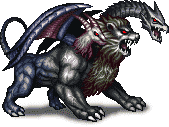
\includegraphics[width=0.3\columnwidth]{./art/monsters/chimera.png}}
{
	HP: & \hfill 70 & MP: & \hfill 100\\
	STR: & \hfill 1 & DEF: & \hfill 2 \\
	MAG: & \hfill 2 & RES: & \hfill 3 \\
	AGI: & \hfill 3 & Size: & \hfill M\\
}
{\accf{Claw}: 2d DMG \hfill \accf{Retaliate} \hfill \accf{Resilient}:\fire\ice\lightning}
{
	\mspell{Firaga}{12}{1r}{Single}{5u}{You deal 6d fire damage to the target.}{\fire}	
	\mspell{Blizzaga}{12}{1r}{Single}{5u}{You deal 6d ice damage to the target.}{\ice}	
	\mspell{Thundaga}{12}{1r}{Single}{5u}{You deal 6d lightning damage to the target.}{\lightning}	
}
%
\vfill
%
\ofmonster{Cactuar}{5}{
\includegraphics[width=0.16\columnwidth]{./art/monsters/cactuar.png}}
{
	HP: & \hfill 25 & MP: & \hfill 60\\
	STR: & \hfill 5 & DEF: & \hfill 0 \\
	MAG: & \hfill 0 & RES: & \hfill 15 \\
	AGI: & \hfill 4 & Size: & \hfill S\\
}
{\accf{Tackle:} 1d DMG \hfill \accf{Auto-Blink}}
{	
	\mtech{1000 Needles}{10}{0r}{Single}{1u}{You deal 10d damage to the target.}{}	
	\mpassive{Flee}{When running away from enemies you can move 2u further than usual.}	
}
%
\newpage
%
\ofmonster{Magic Pot}{5}{
\includegraphics[width=0.16\columnwidth]{./art/monsters/magicpot.png}}
{
	HP: & \hfill 1 & MP: & \hfill 0\\
	STR: & \hfill 0 & DEF: & \hfill 99 \\
	MAG: & \hfill 0 & RES: & \hfill 99 \\
	AGI: & \hfill 1 & Size: & \hfill S\\
}
{	\accf{All-Immune}}
{
	\mreaction{Gimme!}{When given a beneficial Item, you disappear (KO) and drop 1000G. When attacked, make a DC 8 check and upon failure you suffer KO to deal 8d damage in 3u around you, dropping no Gil.}
}
%
\vfill
%
%%%%%%%%%%%%%%%%%%%%%%%%%%%%%%%L6%%%%%%%%%%%%%%%%%%%%%%%%%%%%%%%%%%%%%%%%%
%
%
\ofmonster{Mindflayer}{6}{
\includegraphics[width=0.23\columnwidth]{./art/monsters/mindflayer.png}}
{
	HP: & \hfill 60 & MP: & \hfill 70 \\
	STR: & \hfill 0 & DEF: & \hfill 3 \\
	MAG: & \hfill 5 & RES: & \hfill 4 \\
	AGI: & \hfill 2 & Size: & \hfill M\\
}
{\accf{Staff}: 1d DMG \hfill \accf{Immune}:\poison\silence\sleep \hfill \accf{Resilient}:\water}
{	
	\mspell{Waterga}{14}{1r}{Single}{6u}{You deal 6d water damage to the target.  }{\water}
	\mtech{Mind Blast}{12}{1r}{2u}{5u}{All enemies in the target area suffer 4d dark damage and Immobile for 1 round.}{\immobile \dark}	
}
%
\vfill
%
\ofmonster{Lamia}{6}{
\includegraphics[width=0.24\columnwidth]{./art/monsters/lamia.png}}
{
	HP: & \hfill 65 & MP: & \hfill 50 \\
	STR: & \hfill 3 & DEF: & \hfill 4 \\
	MAG: & \hfill 2 & RES: & \hfill 4 \\
	AGI: & \hfill 3 & Size: & \hfill M\\
}
{\accf{Slap}: 2d DMG \hfill \hfill \accf{Immune}:\poison\sleep\silence \hfill \accf{Weak}:\lightning}
{	
	\mspell{Toad}{16}{1r}{Single}{5u}{
		The target makes a DC 8 check and is turned into a toad upon failure for 3 rounds or until he receives any damage.
		While being a toad, he cannot talk or take any action and can only move 1u per turn.
	}{}	
	\mreaction{Entice}{
		When an enemy successfully Attacks you, he has to make a DC~6 check.
		Upon failure, you can decide which movements and actions he has to perform on his next turn.
	}
}
%
\vfill
%
\ofmonster{Iron Giant}{6}{
\includegraphics[width=0.19\columnwidth]{./art/monsters/irongiant.png}}
{
	HP: & \hfill 130 & MP: & \hfill 80 \\
	STR: & \hfill 7 & DEF: & \hfill 5 \\
	MAG: & \hfill 0 & RES: & \hfill 4 \\
	AGI: & \hfill 2 & Size: & \hfill L\\
}
{\accf{Sword}: 2d DMG, 2u Range \hfill \accf{Counter, Surge}}
{
	\mtech{Sweep}{6}{0r}{3u (front)}{Self}{Make an Attack against all enemies in target area.}{}		
	\mtech{Tremor}{12}{0r}{5u (line)}{Self}{All enemies in the target area make a DC~8 check and upon failure suffer 2d damage, as well as Immobile and DeDEF for 1 round.}{}		
}
%
\vfill
%
\ofmonster{Medusa}{6}{
\includegraphics[width=0.22\columnwidth]{./art/monsters/medusa.png}}
{
	HP: & \hfill 60 & MP: & \hfill 70\\
	STR: & \hfill 3 & DEF: & \hfill 2 \\
	MAG: & \hfill 5 & RES: & \hfill 3 \\
	AGI: & \hfill 3 & Size: & \hfill M\\
}
{\accf{Hair}: 2d DMG \hfill \accf{Immune}:\poison\sleep\immobile \hfill  \accf{Resilient}:\earth\lightning}
{	
	\mtech{Gaze}{16}{0r}{3u (front)}{Self}{Everyone in the target area makes a DC~8 check~and suffers Immobile for 3 rounds upon failure.}{\immobile}	
	\mspell{Thundaga}{12}{1r}{Single}{5u}{You deal 6d lightning damage to the target.}{\lightning}
}
%
\vfill
%
\ofmonster{Ogre}{6}{
\includegraphics[width=0.22\columnwidth]{./art/monsters/ogre.png}}
{
	HP: & \hfill 80 & MP: & \hfill 50 \\
	STR: & \hfill 5 & DEF: & \hfill 3 \\
	MAG: & \hfill 0 & RES: & \hfill 2 \\
	AGI: & \hfill 2 & Size: & \hfill L\\
}
{\accf{Fist}: 2d DMG, 2u Range \hfill \accf{Immnue}:\immobile\destr\dedef}
{	
	\mtech{Beatdown}{5}{0r}{Single}{Weapon}{
		Make an Attack where the target has Advantage on the
		evasion check. If the Attack is successful, you automatically score a Critical Hit.
	}{}
	\mpassive{Change Stance}{
		At the end of each turn you can take one of two stances.
		In offensive stance, you score a Critical Hit, when the target of your Attack rolls 5 or less on the evasion check.
		In defensive stance, when an enemy successfully hits you with an Attack, you can immediately make an Attack on him.
	}
}
%
\vfill
%
%
%%%%%%%%%%%%%%%%%%%%%%%%%%%%%%%L7%%%%%%%%%%%%%%%%%%%%%%%%%%%%%%%%%%%%%%%%%
%
%
\ofmonster{Cerberus}{7}{
\includegraphics[width=0.23\columnwidth]{./art/monsters/cerberus.png}}
{
	HP: & \hfill 100 & MP: & \hfill 100 \\
	STR: & \hfill 5 & DEF: & \hfill 3 \\
	MAG: & \hfill 3 & RES: & \hfill 4 \\
	AGI: & \hfill 3 & Size: & \hfill L\\
}
{\accf{Bite}: 2d DMG \hfill \accf{Counter} \hfill \accf{Resilient}:\fire\ice\lightning}
{	
	\mspell{Firaga}{12}{1r}{Single}{5u}{You deal 6d fire damage to the target. }{\fire}
	\mpassive{Triple Triad}{You can perform each action on up to 3 different targets within its range simultaneously.}
}
%
\vfill
%
\ofmonster{Zu}{7}{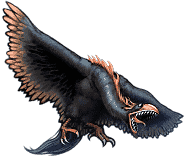
\includegraphics[width=0.25\columnwidth]{./art/monsters/zu.png}}
{
	HP: & \hfill 120 & MP: & \hfill 60 \\
	STR: & \hfill 7 & DEF: & \hfill 5 \\
	MAG: & \hfill 0 & RES: & \hfill 7 \\
	AGI: & \hfill 2 & Size: & \hfill L\\
}
{\accf{Beak}: 2d DMG \hfill \accf{Auto-Regen} \hfill \accf{Immune}:\poison\sleep\silence}
{
	\mtech{Tornado}{10}{1r}{9u (line)}{Self}{
		You create a tornado with a 2u diameter that travels 3u in a line per round for the next 3 rounds.
		Anyone except you that gets into contact with it suffers 4d wind damage and Immobile for 1 round.	
	}{\wind \immobile}	
}
%
\vfill
%
\ofmonster{Sand Worm}{7}{
\includegraphics[width=0.24\columnwidth]{./art/monsters/abyssworm.png}}
{
	HP: & \hfill 105 & MP: & \hfill 110 \\
	STR: & \hfill 5 & DEF: & \hfill 3 \\
	MAG: & \hfill 2 & RES: & \hfill 6 \\
	AGI: & \hfill 1 & Size: & \hfill L\\
}
{\accf{Acid}: 2d DMG, 5u Range \hfill \accf{Resilient:}\earth\wind \hfill \accf{Dual Attack}}
{	
	\mspell{Quake}{18}{1r}{3u}{10u}{Deal 6d+5 earth damage to everyone in the target area.}{\earth}
	\mtech{Inhale}{10}{0r}{Single}{3u}{You inhale the target, removing him from the battle. At the beginning of every turn he may try to free himself by passing a DC 9 check.}{}		
}
%
\vfill
%
\ofmonster{Malboro}{7}{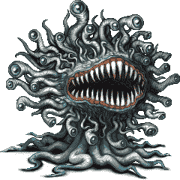
\includegraphics[width=0.24\columnwidth]{./art/monsters/malboro.png}}
{
	HP: & \hfill 140 & MP: & \hfill 125 \\
	STR: & \hfill 6 & DEF: & \hfill 4 \\
	MAG: & \hfill 0 & RES: & \hfill 7 \\
	AGI: & \hfill 2 & Size: & \hfill L\\
}
{
	\accf{Tentacle}: 2d DMG \hfill \accf{All-Immune, Dual Attack}  
}
{
	\mtech{Bad Breath}{12}{0r}{3u (front)}{Self}{
		All enemies in the target area make a DC 8 check and suffer Sleep, Poison, Silence and Blind for 3 rounds upon failure.	
	}{\sleep \poison \silence \blind}	
	\mtech{Gastric Juice}{8}{0r}{2u}{8u}{
		All enemies in the target area suffer 4d damage and make a DC 8 check.
		Every one that fails suffers DeSTR and DeMAG for 5 rounds.	
	}{\destr \demag}
	\mreaction{Entangle}{When you roll higher than 8 on an evasion check, the Attacker suffers Immobile for 1 round upon failure.}
}
%
\vfill
%
\ofmonster{Zombie Dragon}{7}{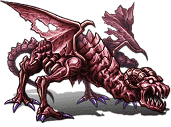
\includegraphics[width=0.31\columnwidth]{./art/monsters/zombiedragon.png}}
{
	HP: & \hfill 115 & MP: & \hfill 90\\
	STR: & \hfill 7 & DEF: & \hfill 5 \\
	MAG: & \hfill 0 & RES: & \hfill 3 \\
	AGI: & \hfill 2 & Size: & \hfill L\\
}
{\accf{Bite}: 2d DMG \hfill \accf{Immune}:\poison\sleep\silence\blind \hfill  \accf{Weak}:\holy \\ \accf{Auto-Regen}}
{
	\mtech{Blindga}{14}{1r}{3u}{5u}{All enemies in the target area make a DC~8 check and suffer Blind for 3 rounds upon failure.}{\blind}	
	\mtech{Poison Breath}{10}{0r}{3u (front)}{Self}{Everyone in the target area suffers 3d damage, makes a DC~8 check~and suffers Poison for 3 rounds upon failure.}{\poison}	
	\mreaction{Rebirth}{Whenever you suffer KO, make a DC~7 check. If you succeed, KO is removed and you regain 50 HP.}	
}
%
\clearpage
%
%%%%%%%%%%%%%%%%%%%%%%%%%%%%%%%L8%%%%%%%%%%%%%%%%%%%%%%%%%%%%%%%%%%%%%%%%%
%
%
\ofmonster{Midgardsormr}{8}{
\includegraphics[width=0.32\columnwidth]{./art/monsters/midgardsormr.png}}
{
	HP: & \hfill 160 & MP: & \hfill 150 \\
	STR: & \hfill 6 & DEF: & \hfill 7 \\
	MAG: & \hfill 0 & RES: & \hfill 5 \\
	AGI: & \hfill 3 & Size: & \hfill L\\
}
{\accf{Tail}: 3d DMG \hfill \accf{Immune:}\poison\immobile \hfill \accf{Counter, Auto-Hit}}
{	
	\mtech{Bite}{4}{0r}{Single}{2u}{Make an Attack against the target. If you hit, the target makes a DC 9 check and also suffers Poison for 3 rounds upon failure. }{\poison}		
	\mtech{Constrict}{6}{0r}{Single}{2u}{Make an Attack against the target. If you hit, the target makes a DC 9 check and also suffers Immobile for 3 rounds upon failure. }{\immobile}	
	\mtech{Burrow}{8}{0r}{2u}{5u}{You burrow into the ground where you cannot be targeted by enemies. At the start of your next turn, you emerge at a location of your choice within 5u and cause 4d damage to all enemies within 2u.}{}
	%\mpassive{Prey}{Whenever you successfully Attack a target that is suffering from a Status Effect, you automatically score a Critical Hit. }					
}
%
\vfill
%
\ofmonster{Behemoth}{8}{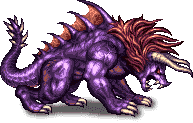
\includegraphics[width=0.31\columnwidth]{./art/monsters/behemoth.png}}
{
	HP: & \hfill 220 & MP: & \hfill 160 \\
	STR: & \hfill 8 & DEF: & \hfill 6 \\
	MAG: & \hfill 6 & RES: & \hfill 5 \\
	AGI: & \hfill 3 & Size: & \hfill L\\
}
{\accf{Claw}: 3d DMG, 2u \hfill \accf{Immune}:\poison\silence \hfill \accf{Resilient:}\fire \\ \accf{Auto-Haste, Counter, Final Attack}}
{
	\mspell{Flare}{20}{2r}{Single}{10u}{You deal 6d+50 damage to the target. The damage dealt ignores the target's RES.}{\fire}	
	\mtech{Heave}{10}{0r}{Single}{2u}{You deal 6d damage to the target and knock him 3u into the air for 1 round.}{}		
}
%
\vfill
%
\ofmonster{Ochu}{8}{
\includegraphics[width=0.3\columnwidth]{./art/monsters/ochu.png}}
{
	HP: & \hfill 170 & MP: & \hfill 140 \\
	STR: & \hfill 7 & DEF: & \hfill 6 \\
	MAG: & \hfill 0 & RES: & \hfill 4 \\
	AGI: & \hfill 2 & Size: & \hfill L\\
}
{\accf{Vines}: 3d DMG, 3u Range \hfill \accf{Resilient:}\water \hfill \accf{Weak:}\fire \\ \accf{Auto-Regen, Dual Attack} \hfill \accf{Immune}:\poison\sleep\silence\blind}
{	
	\mtech{Seed Shot}{8}{0r}{Single}{8u}{The target suffers 6d damage and DeSTR for 1 round.}{}	
	\mtech{Pollen}{15}{0r}{3u}{Self}{All enemies in the target area make a DC 8 check and suffer Sleep and Poison for 3 rounds on failure.}{\sleep \poison}	
	\mpassive{Grappling Vines}{Every target that rolls below 6 on an evasion check against your Attack, suffers Immobile for 3 rounds.}
}
%
\vfill
%
\ofmonster{Red Dragon}{8}{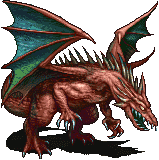
\includegraphics[width=0.24\columnwidth]{./art/monsters/reddragon.png}}
{
	HP: & \hfill 180 & MP: & \hfill 140 \\
	STR: & \hfill 6 & DEF: & \hfill 7 \\
	MAG: & \hfill 5 & RES: & \hfill 5 \\
	AGI: & \hfill 3 & Size: & \hfill L\\
}
{\accf{Bite}: 3d DMG \hfill \accf{Resilient}:\fire \hfill \accf{Immune}:\sleep\blind\immobile \\ \accf{Counter, Surge}}
{
	\mspell{Burn}{12}{0r}{3u (line)}{Self}{The target area is covered in a Hot Field that lasts for 3 rounds.}{\fire}	
	\mtech{Blaze}{14}{1r}{10u (line)}{Self}{You deal 6d fire damage to all enemies in the target area.}{\fire}
	\mpassive{Tail Whip}{Whenever you Attack, you can choose to target all enemies within 1u at once.}	
}
%
\vfill
%
\ofmonster{Vampire Lord}{8}{
\includegraphics[width=0.22\columnwidth]{./art/monsters/vampire.png}}
{
	HP: & \hfill 160 & MP: & \hfill 200 \\
	STR: & \hfill 4 & DEF: & \hfill 5 \\
	MAG: & \hfill 8 & RES: & \hfill 6 \\
	AGI: & \hfill 4 & Size: & \hfill M\\
}
{
	\accf{Bite}: 3d DMG \hfill \accf{Resilient}:\ice\dark\earth \hfill \accf{Weak}:\fire\holy\\
	\accf{All-Immune, Auto-Regen}
}
{
	\mspell{Zombiga}{15}{1r}{Single}{5u}{All enemies in the target area DC~8 check and suffer 4d damage and Zombie for 5 rounds upon failure.}{}	
	\mspell{Blizzaga}{12}{1r}{Single}{5u}{You deal 6d ice damage to the target.}{\ice}	
	\mspell{Curaga}{14}{1r}{2u}{5u}{Everyone in the target area regains 6d HP.}{}	
	\mtech{Bloodsuck}{8}{0r}{Single}{1u}{Make an Attack against the target. If you hit, increase your HP by the amount of damage dealt.}{}
}
%
\vfill
%
%%%%%%%%%%%%%%%%%%%%%%%%%%%%%%%L9%%%%%%%%%%%%%%%%%%%%%%%%%%%%%%%%%%%%%%%%%
%
%
\ofmonster{Tonberry}{9}{
\includegraphics[width=0.28\columnwidth]{./art/monsters/tonberry.png}}
{
	HP: & \hfill 240 & MP: & \hfill 0\\
	STR: & \hfill 15 & DEF: & \hfill 8 \\
	MAG: & \hfill 0 & RES: & \hfill 7 \\
	AGI: & \hfill 2 & Size: & \hfill S\\
}
{\accf{Knife}: 3d DMG \hfill \accf{All-Immune, Revert}}
{	
	\mpassive{Intimidate}{Whenever you move within 3u of an enemy, he makes a DC~8 check and suffers Immobile for 1 round upon failure.}	
	\mpassive{Grudge}{Every time you Attack an enemy, he makes a DC 7 check and suffers KO upon failure. }	
	\mreaction{Karma}{Whenever an enemy that is more than 3u away reduces your HP, deal 6d dark damage back. }
}
%
\clearpage
%
\ofmonster{Kraken}{9}{
\includegraphics[width=0.25\columnwidth]{./art/monsters/kraken.png}}
{
	HP: & \hfill 250 & MP: & \hfill 300 \\
	STR: & \hfill 8 & DEF: & \hfill 6 \\
	MAG: & \hfill 10 & RES: & \hfill 7 \\
	AGI: & \hfill 2 & Size: & \hfill L\\
}
{
	\accf{Tentacle}: 3d DMG, 2u range \hfill \accf{Resilient}:\water\ice\\
	\accf{Auto-Haste, Counter, Dual Attack} \hfill \accf{Immune}:\poison\sleep 
}
{	
	\mspell{Waterga}{14}{1r}{Single}{6u}{You deal 6d water damage to the target.}{\water}	
	\mtech{Ink}{15}{1r}{3u}{6u}{All enemies within the target area make a DC 8 check and suffer Blind and 4d damage upon failure. }{\blind}
	\mtech{Flood}{18}{1r}{100u}{Self}{Everyone on the target area except you suffers 4d water damage. In addition, the target area is covered in a Slow Field for 3 rounds that does not affect you.}{}
}
%
\vfill
%
\ofmonster{Adamantoise}{9}{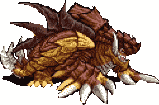
\includegraphics[width=0.32\columnwidth]{./art/monsters/adamantoise.png}}
{
	HP: & \hfill 300 & MP: & \hfill 250 \\
	STR: & \hfill 8 & DEF: & \hfill 7 \\
	MAG: & \hfill 6 & RES: & \hfill 6 \\
	AGI: & \hfill 1 & Size: & \hfill L\\
}
{
	\accf{Trample}: 3d DMG, 2u Target \hfill \accf{Immune}:\poison\silence \\
	\accf{Auto-Regen, Final Attack, Surge} \hfill \accf{Resilient}:\earth
}
{	
	\mspell{Ultima}{28}{2r}{2u}{7u}{You deal 6d+30 dark damage to all enemies in the target area.  }{\dark}	
	\mtech{Roar}{15}{0r}{5u}{Self}{All enemies within the target area make a DC 8 check and suffer Immobile for 3 rounds upon failure. }{\immobile}	
}
%
\vfill
%
\ofmonster{Lich}{9}{
\includegraphics[width=0.28\columnwidth]{./art/monsters/lich.png}}
{
	HP: & \hfill 250 & MP: & \hfill 300\\
	STR: & \hfill 5 & DEF: & \hfill 6 \\
	MAG: & \hfill 12 & RES: & \hfill 8 \\
	AGI: & \hfill 2 & Size: & \hfill L\\
}
{
	\accf{Beam}: 3d DMG, 5u Range \hfill \accf{Resilient}:\dark \\
	\accf{All-Immune, Auto-Regen, Auto-Haste}  
}
{	
	\mspell{Zombiga}{15}{1r}{Single}{5u}{All enemies in the target area DC~8 check and suffer 4d damage and Zombie for 5 rounds upon failure.}{}	
	\mspell{Poisonga}{18}{1r}{3u}{5u}{Everyone in the target area makes a DC 8 check and suffers Poison for 3 rounds upon failure.}{\poison}	
	\mspell{Doom}{18}{0r}{Single}{5u}{The target makes a DC 8 check and suffers KO after 3 rounds upon failure.}{\ko}	
}
%
\vfill
%
\ofmonster{Deathgaze}{9}{
\includegraphics[width=0.3\columnwidth]{./art/monsters/deathgaze.png}}
{
	HP: & \hfill 230 & MP: & \hfill 350 \\
	STR: & \hfill 7 & DEF: & \hfill 6 \\
	MAG: & \hfill 11 & RES: & \hfill 8 \\
	AGI: & \hfill 4 & Size: & \hfill L\\
}
{
	\accf{Claw}: 3d DMG, 2u Range \hfill \accf{Resilient}:\ice \hfill \accf{Weak:}\holy \\
	\accf{All-Immune, Auto-Blink, Auto-Haste}
}
{	
	\mspell{Mega-Doom}{30}{1r}{3u}{5u}{
		All enemies within the target area make a DC~8 check.
		Each target that fails suffers KO after 3 rounds.
	}{\ko}
	\mspell{Blizzaga}{12}{1r}{Single}{5u}{Deal 6d ice damage to the target. }{\ice}		
	\mtech{Retreat}{0}{0r}{Single}{Self}{You make a DC~7 check and if you succeed, you immediately remove yourself from the battle.}{}				
	%\mpassive{Deathtouch}{Whenever you successfully Attack a target, he makes a DC 6 check and immediately suffers KO upon failure.}
	\mreaction{Auto-Dispel}{Whenever an enemy within 5u gains a beneficial Status Effect, you can make a DC 7 check. If you succeed, the Status Effect is immediately removed.}	
}
%
\vfill
%
%%%%%%%%%%%%%%%%%%%%%%%%%%%%%%%L9%%%%%%%%%%%%%%%%%%%%%%%%%%%%%%%%%%%%%%%%%
%
\ofmonster{Ozma}{10}{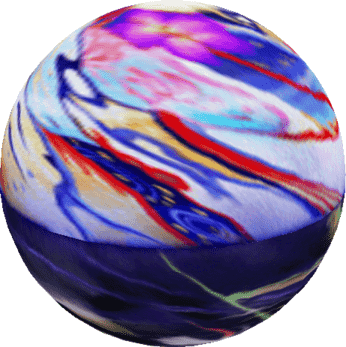
\includegraphics[width=0.23\columnwidth]{./art/monsters/ozma.png}}
{
	HP: & \hfill 300 & MP: & \hfill 400 \\
	STR: & \hfill 4 & DEF: & \hfill 5 \\
	MAG: & \hfill 12 & RES: & \hfill 8 \\
	AGI: & \hfill 2 & Size: & \hfill L\\
}
{
	\accf{Ray}: 4d DMG, 8u Range \hfill \accf{Resilient}:\fire\ice\lightning\earth \\
	\accf{All-Immune, Auto-Haste, Retaliate, CT-0}
}
{
	\mspell{Curaga}{14}{0r}{2u}{5u}{All allies in the target area regain 6d HP.}{}
	\mspell{Thundaja}{18}{0r}{2u}{8u}{Everyone in the target area suffers 6d+15 lightning damage}{\lightning}		
	\mspell{Doomsday}{20}{0r}{2u}{10u}{All enemies in the target area make a DC~6 check and suffer KO upon failure and 6d damage otherwise.}{\earth}				
	\mspell{Curse}{16}{0r}{Single}{5u}{The target makes a DC~8 check and suffers Poison, Silence and Immobile upon failure.}{}	
	\mspell{Absorb MP}{0}{0r}{Single}{10u}{Decrease the target's MP by 4d an increase yours by the same amount.}{}	
	\mreaction{Turbo Counter}{Whenever you suffer damage by an enemy, make a DC~8 check. If you succeed you can take an extra turn immediately after the perpetrator.}
}
%
\vfill
%
\ofmonster{Ruby Weapon}{10}{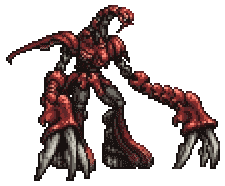
\includegraphics[width=0.3\columnwidth]{./art/monsters/rubyweapon.png}}
{
	HP: & \hfill 400 & MP: & \hfill 300 \\
	STR: & \hfill 12 & DEF: & \hfill 9 \\
	MAG: & \hfill 6 & RES: & \hfill 7 \\
	AGI: & \hfill 2 & Size: & \hfill L\\
}
{
	\accf{Ruby Ray}: 4d DMG, 10u Range \hfill \accf{Resilient}:\earth\dark \\
	\accf{All-Immune, Auto-Regen, Counter, Surge} 
}
{
	\mtech{Whirlsand}{10}{1r}{10u (line)}{Self}{Everyone in the target area is knocked back by 10u and suffers Blind as well as 6d+10 earth damage.}{\earth}				
	\mspell{Ruby Flame}{12}{1r}{Single}{8u}{The target suffers 6d+15 fire damage. The damage dealt is not reduced by the target's RES.}{\dark}
	\mspell{Comet}{18}{1r}{5u}{10u}{Everyone in the target area suffers 6d+10 damage and DeDEF for 3 rounds.}{\dark}
	\mtech{Burrow Tentacles}{8}{0r}{1u}{10u}{You burrow your arms into the ground and two 1u wide tentacles rise from the ground in locations within range, dealing 8d damage to everyone within the target areas.
	While your arms are burrowed, you cannot move and you have to use an action to unborrow them. While burrowed, your tentacles can each perform an Attack (4d DMG) against enemies that are within 3u of them in addition to your usual action on each turn.
}{}	
}
%
\vfill
%
\ofmonster{Chaos}{10}{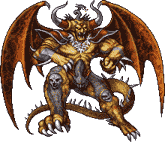
\includegraphics[width=0.26\columnwidth]{./art/monsters/chaos.png}}
{
	HP: & \hfill 400 & MP: & \hfill 400 \\
	STR: & \hfill 9 & DEF: & \hfill 7 \\
	MAG: & \hfill 11 & RES: & \hfill 8 \\
	AGI: & \hfill 3 & Size: & \hfill L\\
}
{
	\accf{Beam}: 4d DMG, 5u Range \hfill \accf{Resilient}:\dark\fire \\
	\accf{All-Immune, Auto-Haste, Retaliate, Revert, Surge}  
}
{	
	\mspell{X-Zone}{13}{0r}{3u}{8u}{You create a Field effect of your choice in the target area that lasts for 3 rounds.}{}		
	\mspell{Ultima}{30}{2r}{50u}{Self}{Deal 6d+40 dark damage to all enemies in the target area.}{\dark}	
	\mspell{Curaja}{20}{1r}{2u}{8u}{All allies in the target area regain 6d+15 HP.  }{}	
	\mspell{Firaja}{18}{1r}{2u}{8u}{You deal 6d+15 fire damage to everyone in the target area.}{\fire}
	\mpassive{Chaos Touch}{Every target that rolls below 6 on an evasion check against your Attack, suffers Blind and Silence for 3 rounds.}
}
%
\vfill
%
\ofmonster{Shinryu}{10}{\includegraphics[width=0.2\columnwidth]{./art/monsters/shinryu.png}}
{
	HP: & \hfill 500 & MP: & \hfill 500 \\
	STR: & \hfill 12 & DEF: & \hfill 9 \\
	MAG: & \hfill 14 & RES: & \hfill 9 \\
	AGI: & \hfill 3 & Size: & \hfill L\\
}
{
	\accf{Tail}: 4d DMG, 4u Range \\
	\accf{All-Immune, Auto-Haste, Auto-Regen, Counter, Retaliate}
}
{
	\mspell{Blizzaja}{18}{1r}{2u}{8u}{Everyone in the target area suffers 6d+15 ice damage}{\ice}		
	\mspell{Tidal Wave}{22}{1r}{10u (front)}{Self}{All enemies in target area take 6d+10 water damage and suffer Immobile for 2 rounds.}{\water \immobile}	
	\mspell{Atomic Rays}{20}{1r}{8u}{Self}{All enemies in the target area take 6d fire damage and suffer Poison for 3 rounds.}{\fire \poison}		
	\mpassive{Adapt Element}{
		At the start of every turn, choose one element (e.g. fire). 
		You gain Resilience against the element until the start of your next turn.
	}
}
%
\vfill
%
\ofmonster{Omega}{???}{\includegraphics[width=0.3\columnwidth]{./art/monsters/omega.png}}
{
	HP: & \hfill 999 & MP: & \hfill 999 \\
	STR: & \hfill 19 & DEF: & \hfill 11 \\
	MAG: & \hfill 17 & RES: & \hfill 10 \\
	AGI: & \hfill 4 & Size: & \hfill L\\
}
{
	\accf{Laser}: 4d DMG, 10u Range \hfill \accf{Resilient}:\fire\dark\lightning \\
	\accf{All-Immune, Auto-Blink, Auto-Haste, Auto-Regen, Counter, Dual Attack, Revert, Retaliate, Surge}
}
{	
	\mspell{Meltdown}{30}{1r}{10u}{Self}{A system vulnerability forces you to leak restricted memory content and lava. Deal 6d+40 fire damage on the target, including yourself.}{\fire}	
	\mtech{Biohazard}{16}{0r}{3u}{10u}{All enemies in the target area make a DC~8 check and suffer Poison, Blind and Slow for 3 rounds.}{\fire}
	\mtech{Flamethrower}{8}{0r}{3u (front)}{Self}{Deal 6d+10 fire damage to all enemies in the target area. Also, the target area is covered in a Hot Field for 3 rounds.}{\fire}
	\mtech{Wave Cannon}{14}{1r}{3u}{12u}{You inflict 6d+20 dark damage and DeDEF, DeRES and DeSTR for 5 rounds on the target area. }{\dark \dedef \deres}		\\
	\vspace*{-0.2cm}\\
	\ofquote{”Man forges a weapon to fell the gods: Omega. The weapon knows nothing of compassion - only destruction! Its might knows no equal. The wise dare not cross its path, lest they meet their end.”}{Gentiana}
}
%
%
\clearpage